%%
\chapter{Case Demonstrations} \label{ch:case}

\section{Introduction}

As suggested by the information content analysis in last chapter, 
adding polarization data into the AERONET inversion will enable the 
retrieval of bi-modal refractive index and SSA even for 440-nm AOD as 
low as 0.2 when the Ångström exponents (AE) is between 0.7 and 1.6. 
We also found that the uncertainty in the retrieval can be reduced by up 
to 79\% (57\%), 76\% (49\%), 69\% (52\%), 66\%
(46\%), and 49\% (20\%) for the fine-mode (coarse-mode) $V_0$, $\reff$,
$\reff$, $\mreal$, and SSA, respectively. 
In this chapter, our new research algorithm is applied to a suite of 
photo-polarimetric measurements taken from the new-generation SunPhotometer 
at the Beijing\_RADI AERONET station. I present the selected cases and the
\textit{a priori} characterizaton in section \ref{sec:case}, and discuss the 
fitting residuals in section \ref{sec:invfit} and the retrieved 
results in section \ref{sec:inv0}. A contrast analysis is presented in section
\ref{sec:inv1} to demonstrate the superiority of the 
inversion involving polarization.

\section{Selected Cases and the \textit{a priori} Characterization}
\label{sec:case}

We applied our algorithm to the radiance and polarization measured by the CIMEL
CE318-DP SunPhotometer (instrument \#350) at Beijing\_RADI (116.37$^\circ$E,
40.00$^\circ$N), which is a joint station of the AERONET and the 
Sun/sky-radiometer Observation NETwork (SOnet). The AOD measurements are 
designated from the field-calibrated level 1.5 products. Measurements of the 
direct and diffuse radiance as well as DOLP were performed at eight spectral 
wavelengths, with the measurements at 440, 675, 870, and 1020 nm chosen for 
the inversion. The sky radiances were calibrated following \citet{Li08} and 
are reported as values normalized by the extra-terrestrial solar irradiance. 
The DOLP were calibrated in the laboratory following \citet{Li10}. 
Measurement uncertainties were estimated to be 0.01--0.02 for AOD, 3--5\% for 
radiance, and 0.01 for DOLP.

%% Figure aerosol climatology
\begin{figure}[p]
  \centering
  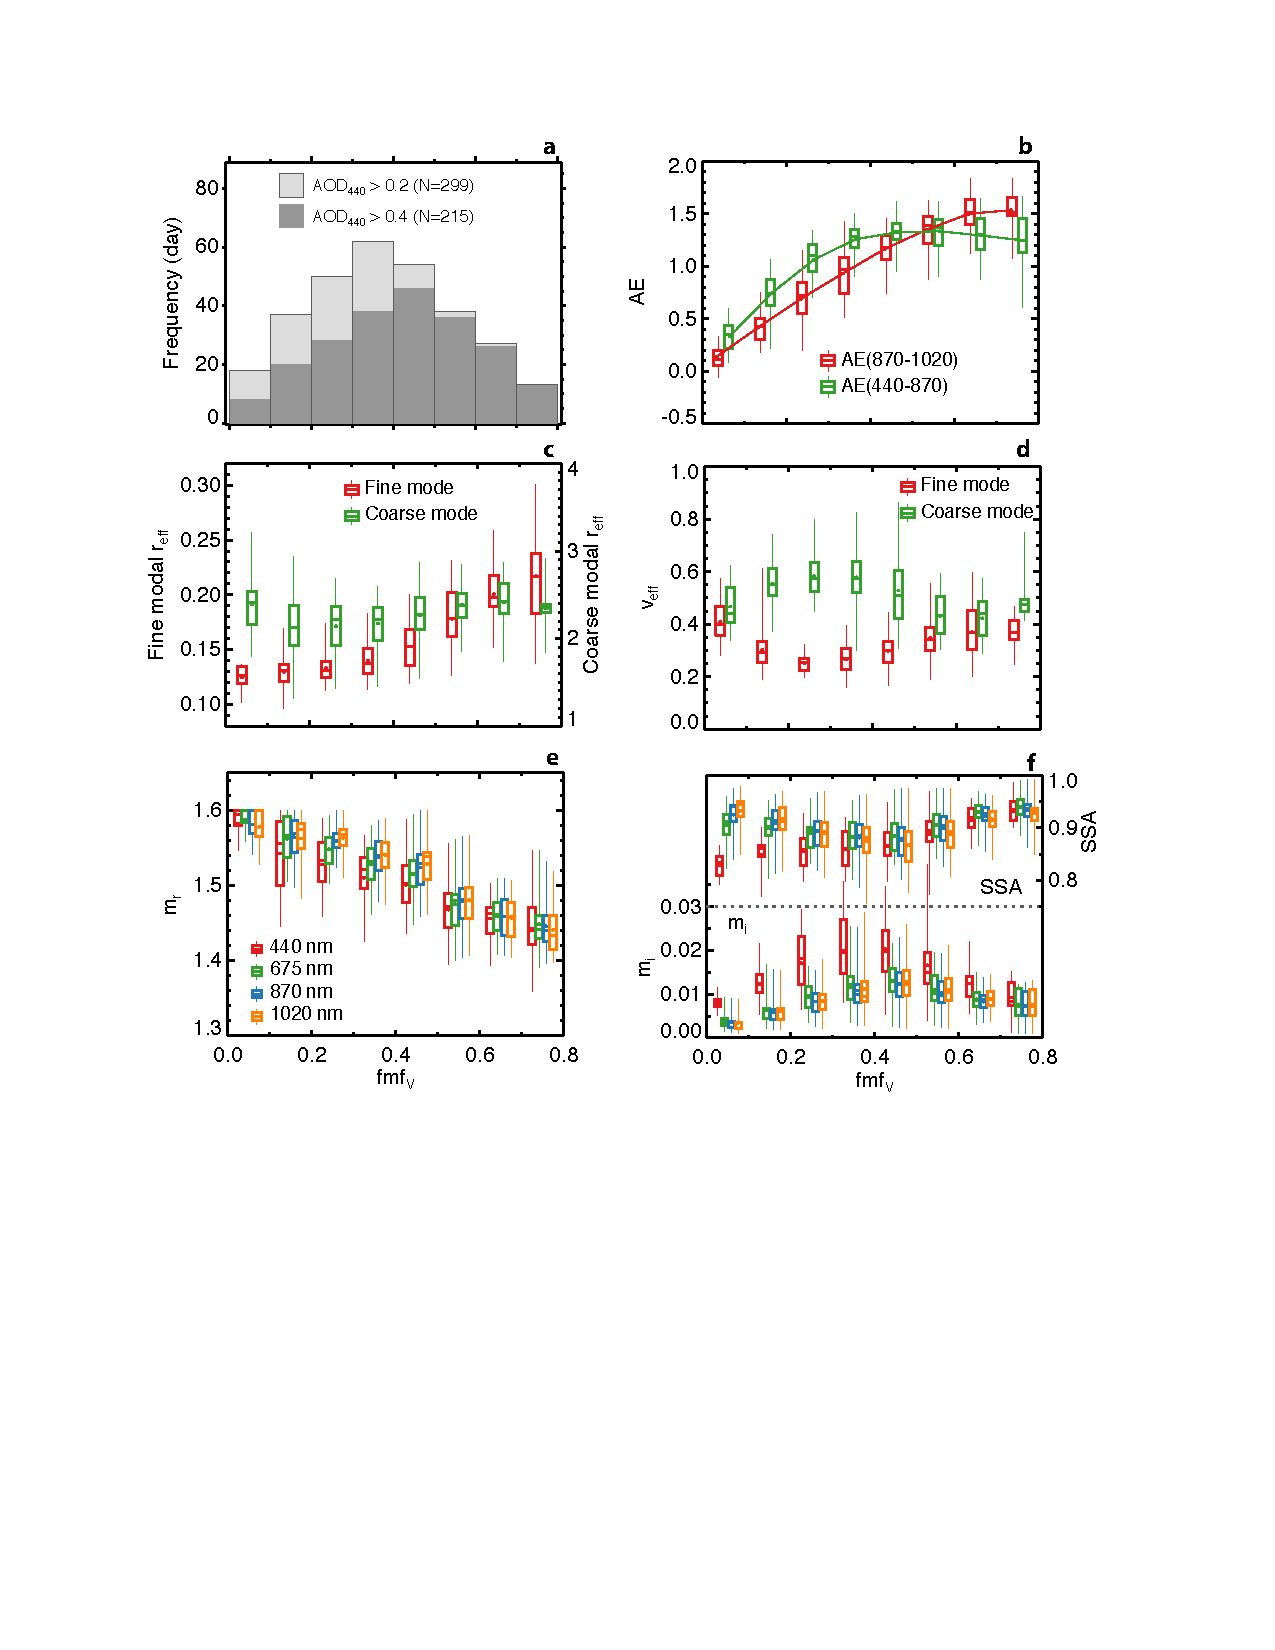
\includegraphics[width={\textwidth}]{figures/inv01.pdf}
  \caption{Climatology of aerosol properties over the Beijing\_RADI site derived
from AERONET daily inversion products during 2011--2013. The variables are shown
as functions of the fine-mode-fraction in terms of the aerosol volume, or
$\fmfv$. Eight bins are applied for $\fmfv$ from 0 to 0.8 with an increment of 0.1.
The six panels are: (a) Histogram of used data; (b) the Ångström exponents (AE)
derived from from 870 to 1020 nm (red) and from 440 to 870 nm (green)
wavelength pairs; (c) the effective radius for aerosols in the fine (red) and
coarse (green) mode; (d) the effective variance in the fine (red) and coarse
(green) mode (green); (e) the real part of the refractive index at 440, 675,
870, and 1020 nm; and (f) the imaginary part of the refractive index and
aerosol SSA at the same wavelengths.}
  \label{fig:invap}
\end{figure}

%% Selected case
\begin{table}[b]
  \centering
  \small
  \caption{Main characteristics of case studies in this work.}
  \label{tab:invcase}
  \begin{tabular}{p{2em} C{7em}  C{4em} C{2em} C{5em} C{4em} C{4em} C{2em}}
  \toprule
  Case  & Date \& Time \newline UTC& $\theta_0(^\circ)$ & ${\taua}_{440}$ &
  AE\newline(870/1020nm)& OMI \ce{NO2} \newline(molec/cm$^2$) & 
  OMI \ce{O3} \newline (DU) & Vapor \newline (cm) \\
  \midrule
   A & 02/22/2011 04:30	& 50.3--50.6 & 3.46 & 1.57 & 6.3$\times$10$^{16}$ & 356.5 & 0.86\\
   B & 03/17/2013 03:25 & 43.0--42.2 & 2.74 & 1.39 & 4.2$\times$10$^{16}$ & 332.7 & 0.76\\
   C & 03/22/2013 07:23 & 57.0--60.0 & 1.05 & 1.01 & 4.1$\times$10$^{16}$ & 386.7 & 1.01\\
  \bottomrule
  \end{tabular}
\end{table}

The \textit{a priori} is characterized with the climatology of aerosol properties
derived from the version 2.0 AERONET daily inversion products of the same site
during 2011--2013. The PSD parameters were analyzed with 299 available daily
inversions when the 440-nm AOD is larger than 0.2. The refractive index and SSA
were analyzed with 215 inversions when the 440-nm AOD is larger than 0.4. In
Figure \ref{fig:invap}, the variables are shown as functions of the 
fine-mode-fraction in terms of the aerosol volume, or $\fmfv$. It can be found 
that the $\fmfv$ from 0.2 to 0.6 accounts for $\sim$70\% of occurrences (Figure
\ref{fig:invap}a), indicating aerosol over this site is dominated by the mixed 
fine-coarse aerosols. The AE derived from the 1020-nm and 870-nm AOD pairs is 
more linearly related to the $\fmfv$ than the 440-nm and 870-nm AE (Figure
\ref{fig:invap}b), because AE over the longer-wavelength pairs is more
sensitive to the component fraction and less sensitive to the change of
component particle size \citep{Schuster06}. From Figure \ref{fig:invap}c--f, 
we determine the a priori ($\xabf$) based on the corresponding mean values. 
For refractive index, we pick their mean values when $\fmfv<0.2$ for the coarse
mode and when $\fmfv>0.6$ for the fine mode. The \textit{a priori} error 
($\epsilon\uda$) for each parameter is determined by the relevant physical 
range, and is listed in the last column of Table \ref{tab:inverr}. 
In addition, we found in the Figure \ref{fig:invap}e that the $\mreal$ 
retrievals decrease quasi-linearly with the increasing $\fmfv$, which indicates
the $\mreal$ has distinct values between aerosols in the fine and the coarse
modes over this site. It is expected that, the $\mreal$ in the mixed aerosol
situations, e.g., $0.3<\fmfv<0.6$, is also expected to have the separated 
values for fine- and coarse-mode particles.

With the above \textit{a priori} characterization, we performed retrievals for three
cases, respectively, on 22 February 2011, 17 March 2013, and 22 March 2013
(hereinafter, cases A, B, and C). A brief characterization of these cases is
presented in Table \ref{tab:invcase}. Indeed, these cases represent different 
aerosol mixtures: (A) dominated by fine particles, (B) well-mixed, and (C) 
dominated by large particles. Moreover, the present algorithm is designed to 
run with two inversion scenarios: the first includes DOLP, while the second ignores
it---hereafter, we label these scenarios type P and I, respectively. An
examination of the difference in the fitting results between these two types of
inversion would indicate the value of DOLP in improving the retrieval. For all
cases, optimal solutions are achieved within less than thirty iterations, and
further iterations yield negligible reduction of the cost function. 

\section{Fitting Residuals} \label{sec:invfit}

The fitting residual characterizes the disagreement between the model and the
measurement. The individual sky radiance residual is defined as a relative
quantity: 
\begin{equation}
e_\text{I}=(I_\text{calc}-I_\text{meas})/I_\text{meas}
\end{equation}
where $I_\text{calc}$ and $I_\text{meas}$ denote the calculated (using the 
retrieved aerosol parameters) and measured sky radiances, respectively. 
In contrast, the fitting residuals for AOD and DOLP are defined by: 
\begin{align}
e_\text{AOD} &= \text{AOD}_\text{calc}-\text{AOD}_\text{meas}, \\
e_\text{DOLP} &= \text{DOLP}_\text{calc}-\text{DOLP}_\text{meas}.
\end{align}
The residual errors for AOD, sky radiance, and DLOP are mean values of
$|e_\text{I}|$, $|e_\text{AOD}|$, and $|e_\text{DOLP}|$, respectively.

%% Figure of Fitting residual
\begin{figure}[t]
  \centering
  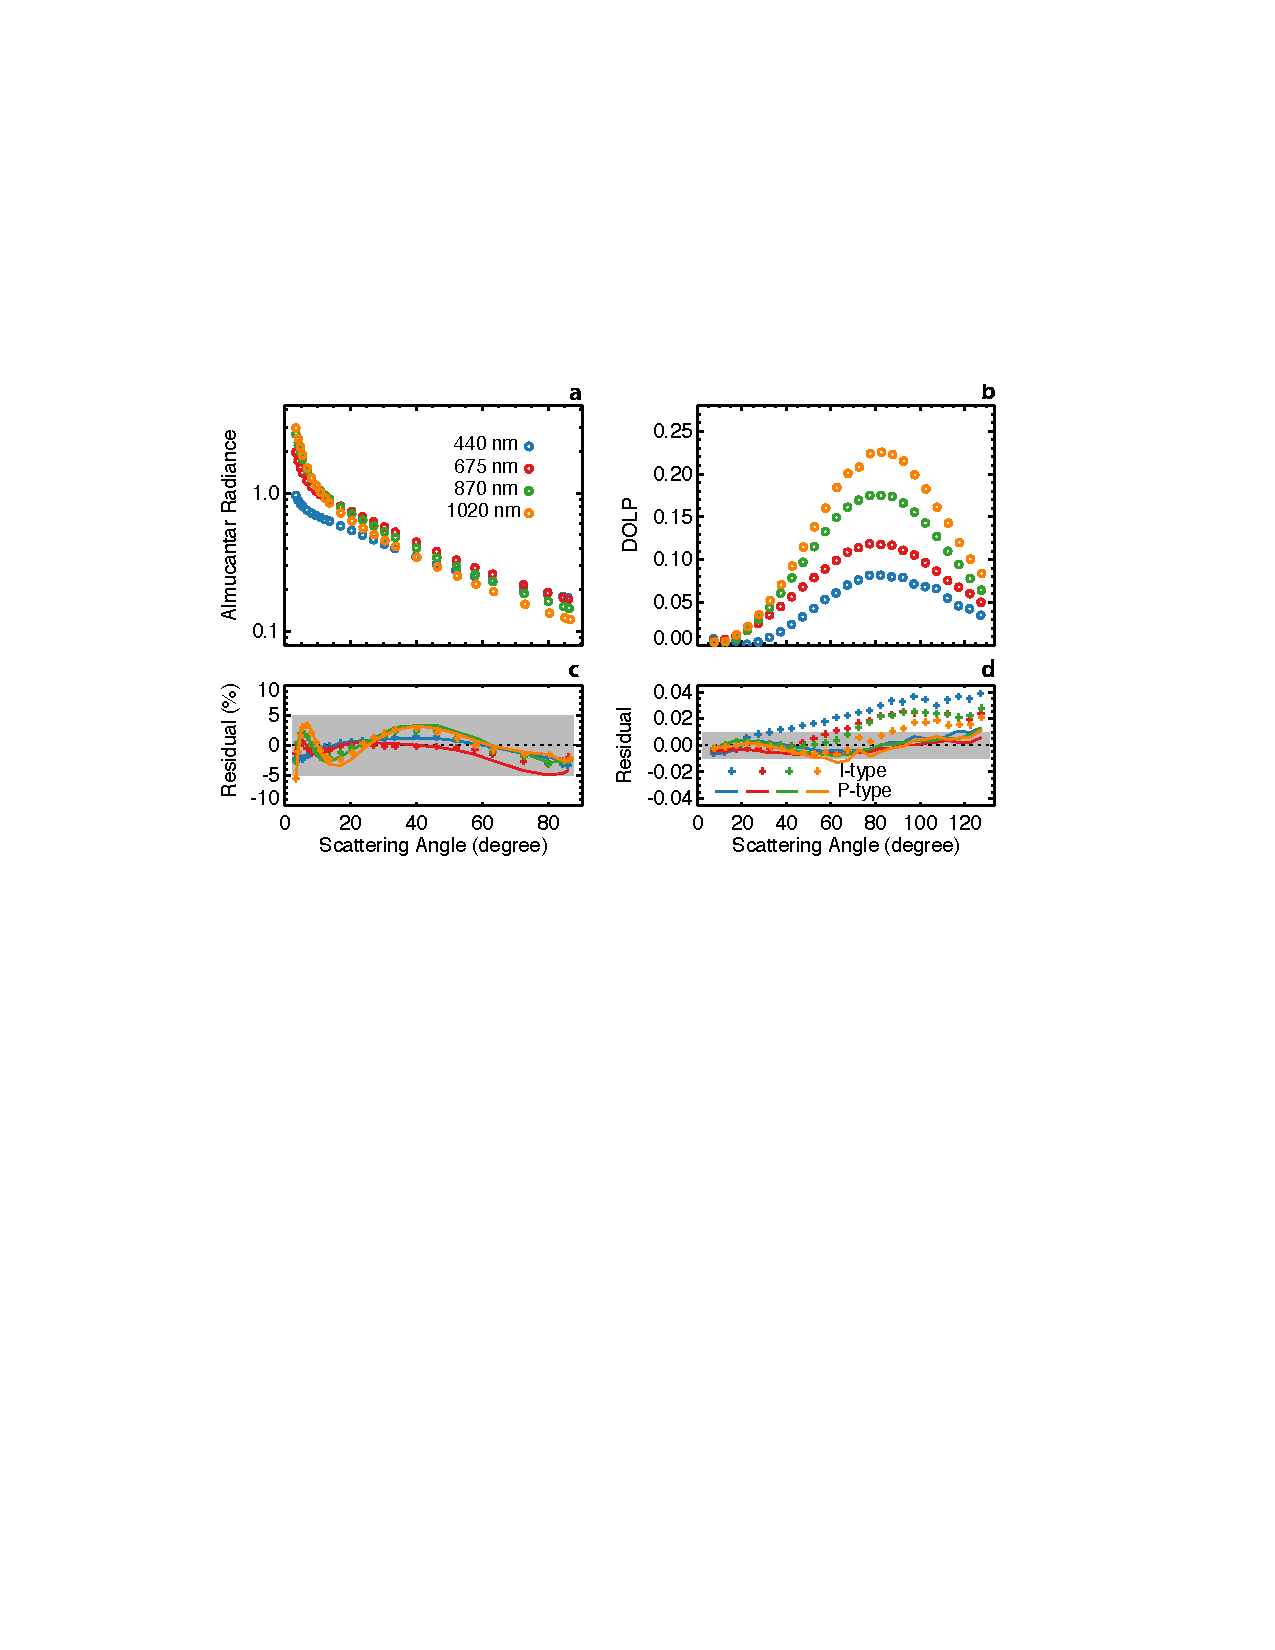
\includegraphics[width={\textwidth}]{figures/inv02.pdf}
  \caption{a) Measured almucantar normalized radiances. (b) Measured DOLP in
the solar principal plane. (c) Fitting residuals for almucantar radiances by
the P-type inversion (solid curves) and I-type inversion (crosses). (d) Same as
panel (c), but for fitting the residuals of principal-plane DOLP. Four colors
indicate different wavelengths: blue for 440 nm, green for 675 nm, red for 870
nm, and orange for 1020 nm. Gray areas in panels c–d indicate the measurement
uncertainty.}
  \label{fig:invfit}
\end{figure}

Because similar fitting results are found for these three aerosol types
(cases), we illustrate in Figure \ref{fig:invfit} the fitting results for sky 
radiances and DOLP only for the case B. The statistical residual errors are 
displayed in Table \ref{tab:invfit} for all three cases. We found that 
retrievals from both types of inversion can well reproduce these AERONET 
measurements of AOD and sky radiances. Fitting residuals from both types of 
inversions for individual ALM radiance measurement lie within the experimental
uncertainty of 5\%, although the fit of radiances from the P-type inversion 
is slightly deteriorated: residual error is 1.67\% for the P-type compared
1.43\% for the I-type inversion. However, the DOLP residual
error can be much larger for the I-type inversion than that for the P-type
inversion: 0.014 versus 0.004. As these fitting results show, without the
constraints imposed by polarization, the retrieved aerosol microphysical
parameters could result in larger error in polarization simulations,
highlighting the necessity to include polarization in the inversion as an
additional source of constraint. 

%% Fitting residuals
\begin{table}[t]
  \centering
  \small
  \caption{Summary of measurement fitting errors.}
  \label{tab:invfit}
  \begin{tabular}{p{3em} C{6em}  C{6em} C{6em} C{6em}}
  \toprule
  Case &  Inversion type & AOD \newline residual error & 
    Radiance \newline residual error & DOLP \newline residual error \\
  \midrule
   A & I & 0.0005 & 1.68\% & 0.008 \\
     & P & 0.0010 & 1.78\% & 0.005 \\
   B & I & 0.0003 & 1.43\% & 0.014 \\
     & P & 0.0003 & 1.67\% & 0.004 \\
   C & I & 0.0007 & 2.77\% & 0.027 \\
     & P & 0.0034 & 3.73\% & 0.009 \\
  \bottomrule
  \end{tabular}
\end{table}

\section{Retrieved Aerosol Properties} \label{sec:inv0}

Figure \ref{fig:inv01} displays our retrievals from both I-type and P-type 
inversions for the aerosol volume PSD and complex refractive indices. 
Also shown are the retrievals from the AERONET \Dub inversion. 
Table \ref{tab:invpsd} presents the values of the (P-type inversion) retrieved
PSD parameters including $V_0$, $\reff$, $\veff$, $\rv$, and $\sg$ for both 
fine and coarse modes, and corresponding values from the \Dub inversion. 
The PSD in these cases consists separated fine and coarse aerosol modes. 
In the cases dominated by fine-mode aerosol (A) and
well-mixed aerosol (B), our retrievals agree with the AERONET inversions,
though marginal differences are found in the effective radius and standard
deviation. In case C dominated by coarse-mode aerosols, our algorithm results
in a smaller coarse mode $\reff$ than that from the AERONET algorithm; this may
be caused by our assumption of spherical particles, whereas the \Dub
algorithm considers non-sphericity for coarse particles. We did not find
significant differences in the aerosol volumes between our algorithm and the
\Dub algorithm. As Figure \ref{fig:inv01}b--c indicate, fine-mode volume 
retrieved by the P-type inversion is lower than that retrieved by the 
I-type inversion; such an overestimation from radiance-only inversion was 
also found by \citet{Li09}.

%% Figure retrieval of PSD, refractinve index
\begin{figure}[t]
  \centering
  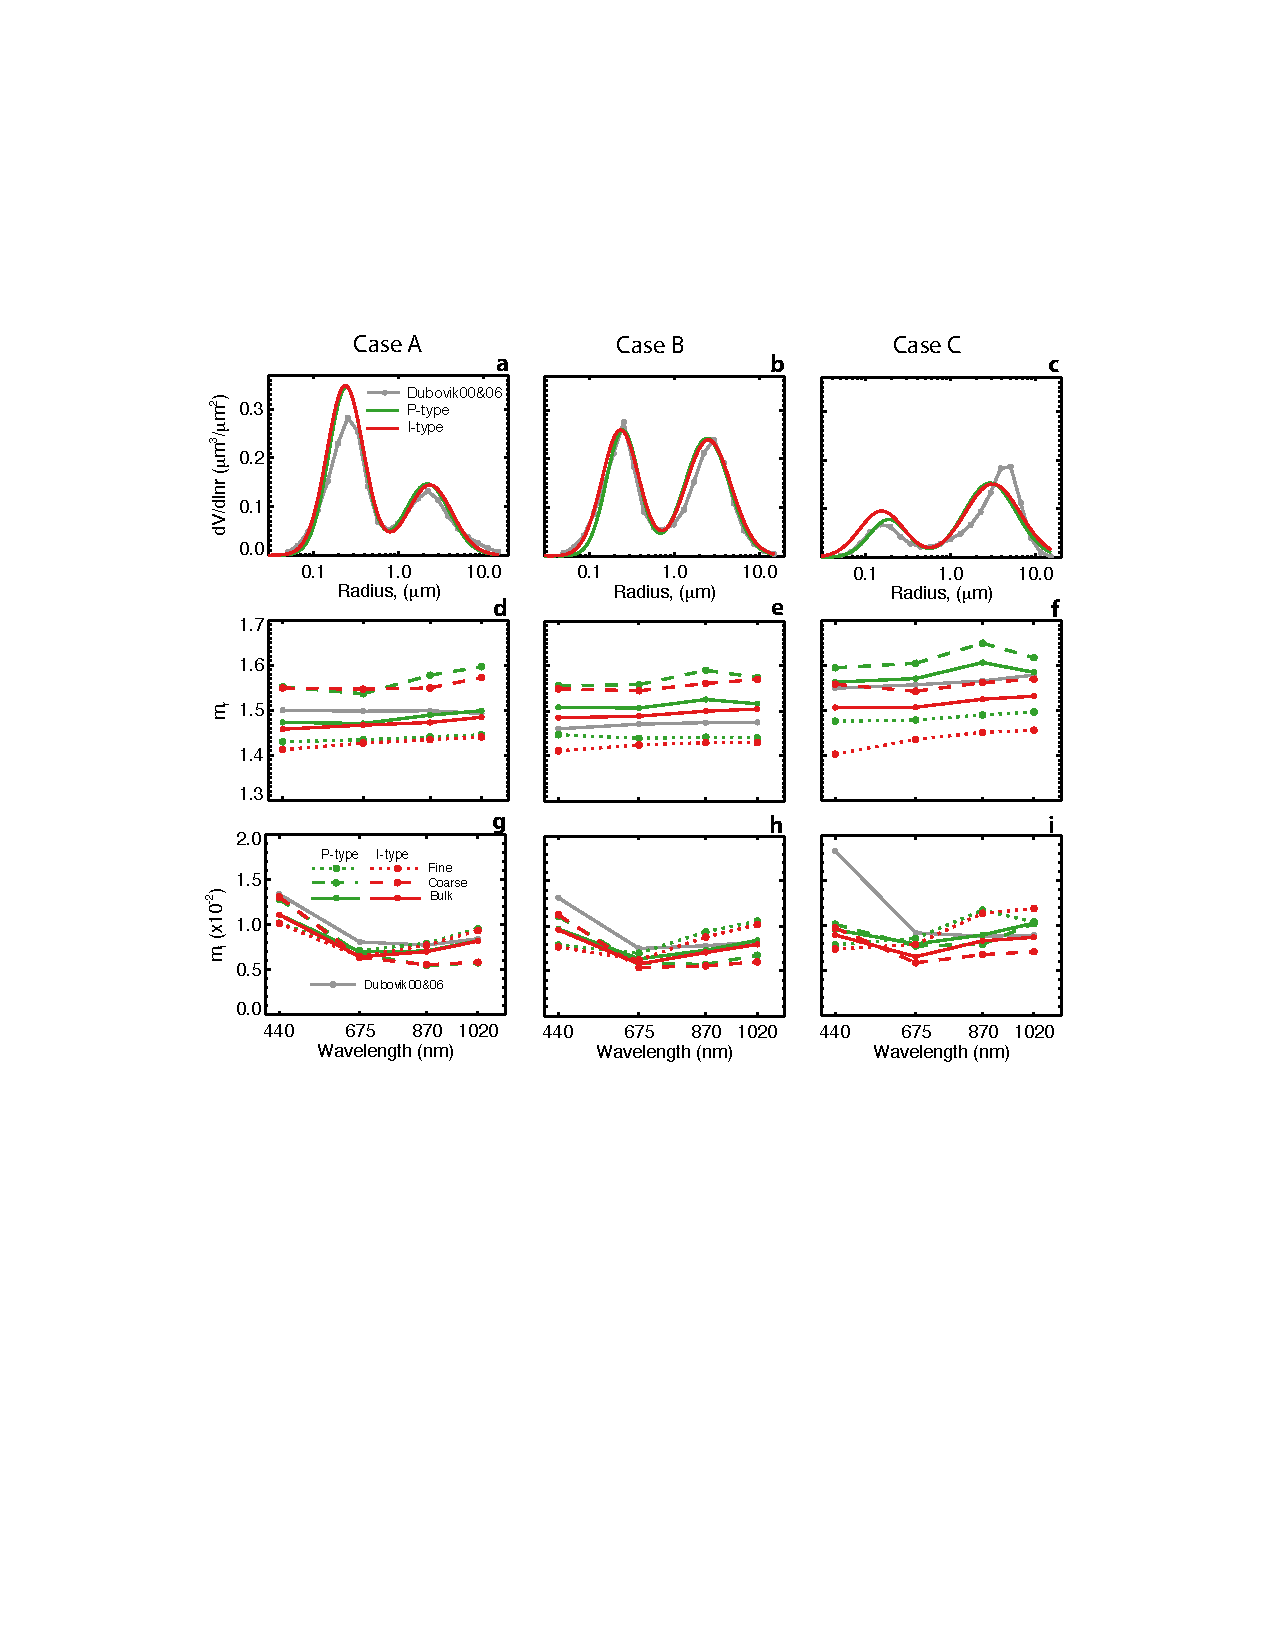
\includegraphics[width={\textwidth}]{figures/inv03.pdf}
  \caption{Retrieved aerosol volume size distribution (PSD) and refractive
index compared with \Dub inversions (gray). P-type and I-type
inversions are represented by green and red colors, respectively. In panels
d--i, the retrievals are shown for aerosols in both fine (dotted) and coarse
(dashed) modes, as well as bulk averages (solid). The PSD relevant quantities
for panels a--c are summarized in Table \ref{tab:invpsd}.}
  \label{fig:inv01}
\end{figure}

%% Figure retrieval of SSA and asy
\begin{figure}[t]
  \centering
  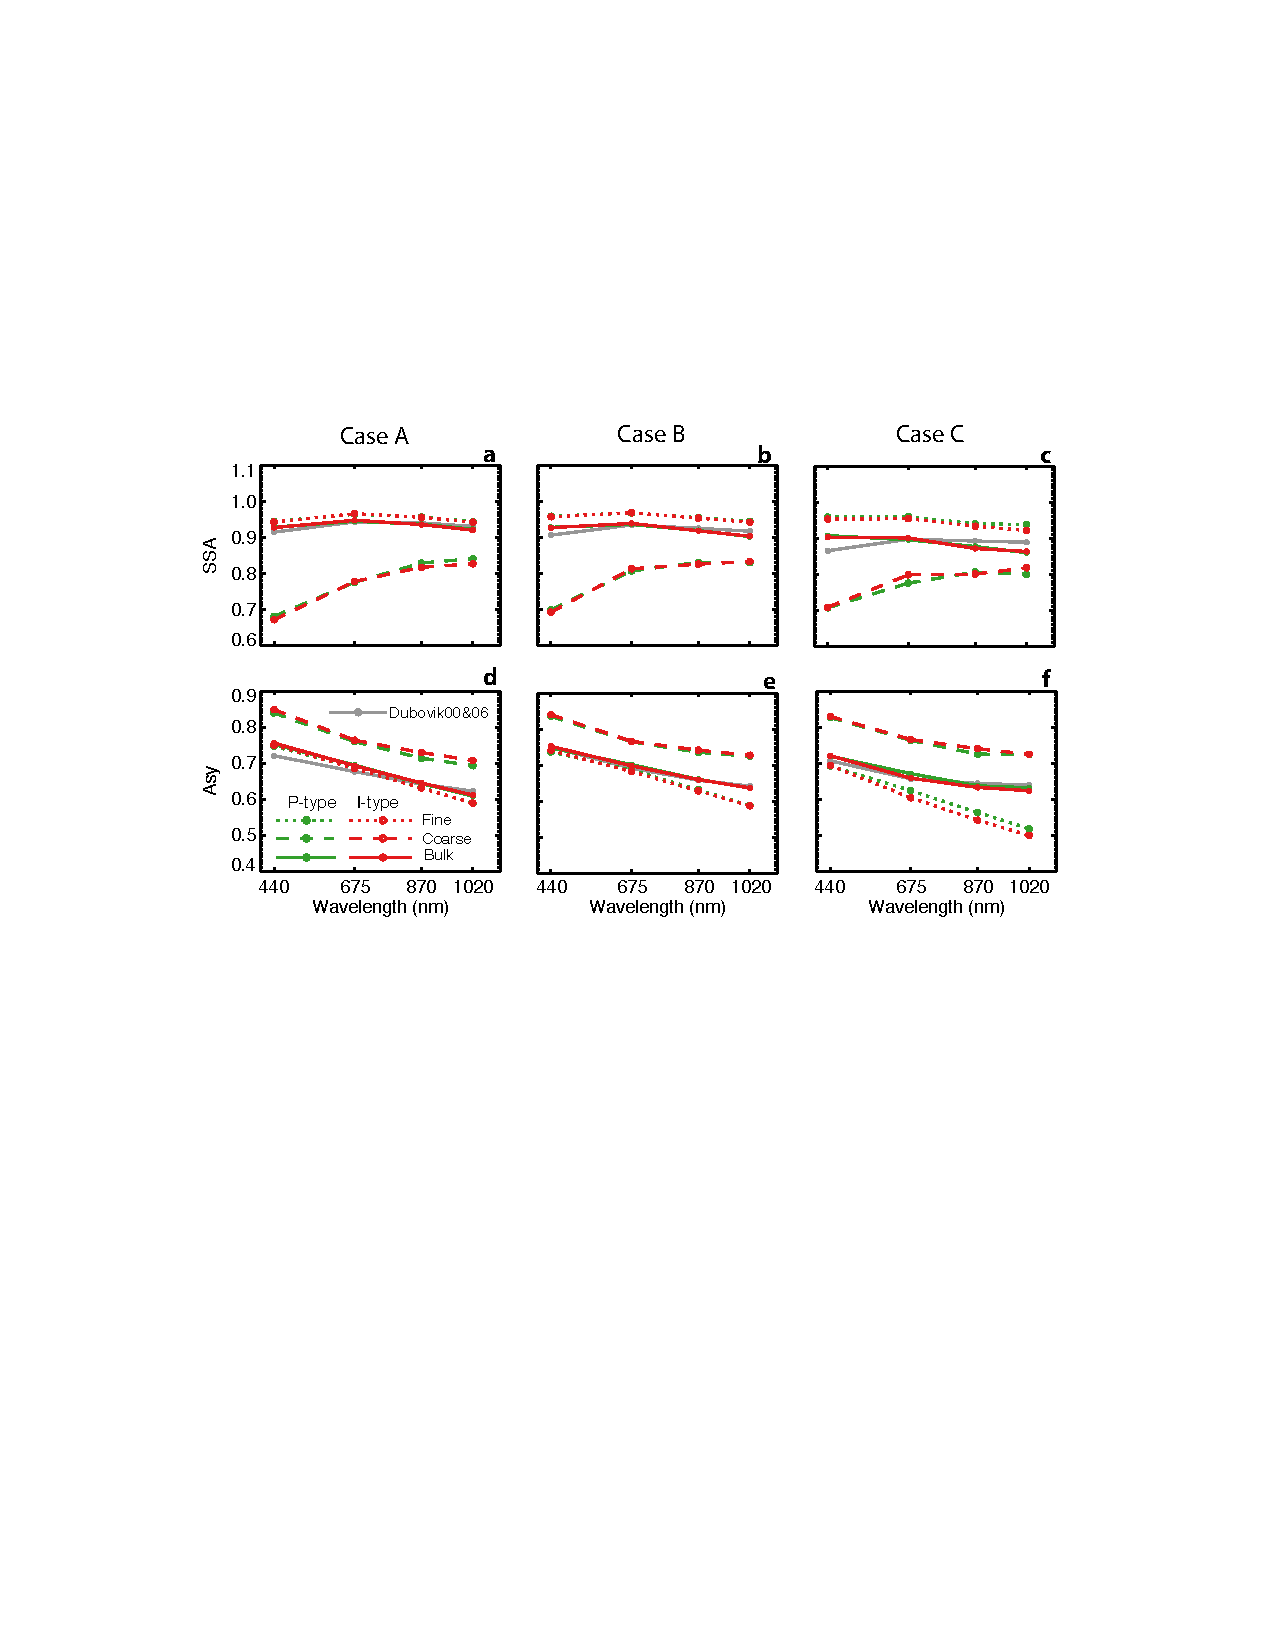
\includegraphics[width={\textwidth}]{figures/inv04.pdf}
  \caption{Same as Figure \ref{fig:inv01}, but for derived aerosol SSA and Asy.}
  \label{fig:inv02}
\end{figure}

In contrast with the \Dub algorithm, which retrieves a single
refractive index for each spectrum that is independent of aerosol size, our
retrieved aerosol refractive indices are pertain to the corresponding fine and
coarse modes. In order to get a general impression of the agreement between our
retrievals and the AERONET inversions, we compute the bulk refractive index
that is a weighted average by the particle volume of each mode in our retrieval
\citep[e.g.,][]{Wang07}. According to Figure \ref{fig:inv01}d--f, while the 
bulk value of $\mreal$ is in good agreement (differences $<$ 0.03) with that of
the \Dub retrievals, our retrieval allows for a mode-resolved characterization
 of aerosol refractive index. For instance, the aerosol $\mreal$ has values 
1.5--1.6 in the coarse mode, which is larger than that in the fine mode (1.4--1.5).
In addition, we found that the P-type inversion usually yields higher values of
$\mreal$ compared to the I-type inversion; this finding agrees with \citet{Li09}
in that the radiance-only inversion underestimates $\mreal$. 

%% Table of retrieval results
\begin{table}[t]
  \centering
  \small
  \caption{PSD-related parameters retrieved by our P-type inversion, compared
with values from the AERONET \Dub inversion. }
  \label{tab:invpsd}
  \begin{tabular}{p{2em} C{4em} R{3em} R{4em} R{3em} R{4em} R{3em} R{4em}}
  \toprule
  & & \multicolumn{2}{c}{Case A} &
      \multicolumn{2}{c}{Case B} & 
      \multicolumn{2}{c}{Case C} \\
  \cmidrule(r){3-8}
  $\xbf$ &  Units & Ours & AERONET & Ours & AERONET & Ours & AERONET \\
  \midrule
  $V_0\fine$     & $\vunit$ & 0.41  & 0.36  & 0.29  & 0.31  & 0.10  & 0.09  \\
  $\reff\fine$   & $\runit$ & 0.218 & 0.208 & 0.226 & 0.201 & 0.163 & 0.156 \\
  $\veff\fine$   &  --      & 0.25  & 0.32  & 0.22  & 0.32  & 0.31  & 0.33  \\
  $\rv\fine$     & $\runit$ & 0.243 & 0.240 & 0.249 & 0.232 & 0.186 & 0.179 \\
  $\sg\fine$     &  --      & 1.60  & 1.69  & 1.56  & 1.69  & 1.68  & 1.70  \\
  \hline
  $V_0\coarse$   & $\vunit$ & 0.22 & 0.21 & 0.37 & 0.32 & 0.27 & 0.26 \\
  $\reff\coarse$ & $\runit$ & 1.83 & 2.01 & 2.02 & 2.26 & 2.26 & 2.61 \\
  $\veff\coarse$ & --       & 0.44 & 0.53 & 0.45 & 0.38 & 0.65 & 0.50 \\
  $\rv\coarse$   & $\runit$ & 2.20 & 2.44 & 2.44 & 2.65 & 2.91 & 3.28 \\
  $\sg\coarse$   & --       & 1.83 & 1.92 & 1.84 & 1.76 & 2.03 & 1.89 \\
  \bottomrule
  \end{tabular}
\end{table}

According to Figure \ref{fig:inv01}g-–i, the bulk $\mimag$ retrieved by our
algorithm is consistent overall with that from the \Dub algorithm, with both 
retrievals showing similar spectral dependencies. One exception is for case C;
$\mimag$ at 440 nm is about 0.01 from our algorithm but is about 0.02 with the
\Dub algorithm. As expected, our inversion algorithm also offers mode-resolved
$\mimag$. We notice in our retrieval that $\mimag$ shows an increasing 
dependence on the spectral wavelength for the fine mode but a decreasing 
tendency for the coarse mode. 

In the forward modeling framework, the aerosol macrophysical optical properties
act as intermediate model parameters to link the aerosol microphysical
characteristics to the radiation fields. These macrophysical optical parameters
include but are not limited to the aerosol SSA ($\assa$), the scattering phase
function, and the asymmetry factor (Asy). These quantities do not appear in the
state vector; instead, they can be derived from the retrieved microphysical
parameters, and are thus called derived or intermediate parameters. In Figure
\ref{fig:inv02}, we present $\assa$ and Asy from our retrieval, and the 
comparison with their counterparts from the \Dub inversion. In our retrieval,
bulk values of $\assa$ and Asy are again calculated by a scatter-weight 
averaging of the fine and coarse mode values. We found that the bulk $\assa$ 
and Asy from our algorithm and the \Dub algorithm agree very well. 
However, our retrieved coarse-mode $\assa$ varies from 0.7 to 0.9, increasing
with wavelength. In contrast, the retrieved fine-mode $\assa$ runs close to 0.9. 

\section{Improvement over Radiance-Only Retrievals} \label{sec:inv1}

The above comparisons of retrieval results confirm that both P- and I-type
inversions by our algorithm can generate solutions quite consistent with the
current \Dub algorithm. In order to demonstrate the improvements in the
retrieval by including polarization, we compare the retrieval errors between
the P-type and I-type inversions in Table \ref{tab:inverr} for individual aerosol parameters.
Also compared are the errors in the derived $\assa$ and Asy. Clearly, the P-type
inversion yields lower retrieval errors for all the retrieved and derived
parameters; this is confirmed by the theoretical analysis in Chapter
\ref{ch:info} of this thesis. The key points from the comparison are:

(i) Polarization measurements provide important constraints in improving the
retrieval of $V_0$, $\reff$, and $\veff$ for both fine and coarse aerosol modes. For
these three cases, the errors in the retrieved $V_0$ with polarization are less
than 3\% for the fine mode and less than 5\% for the coarse mode, representing a
significant decrease from their counterparts ($\sim$15\% and $\sim$10\%) in the I-type
inversion. Adding polarization can also decrease the error in $\reff$ of both
fine and coarse modes from 10--15\% for the I-type inversion to 3\% and below.
Errors in $\veff$ retrieved by the P-type inversion are 9--11\% for aerosol in the
fine mode and 17--26\% in the coarse mode, whereas they can exceed 60\% with the
I-type inversion.

(ii) Polarization measurements also provide useful constraints in improving the
refractive index retrievals. The most significant improvement is found in the
fine-mode $\mreal$, where the error is lower than 0.01 for the P-type inversion,
compared to 0.02--0.04 for the I-type inversion. The error in the coarse-mode
$\mreal$ from P-type inversion ranges from 0.04 to 0.11, depending on the prevalence
of coarse-mode particles. For retrieving $\mimag$, the inclusion of polarization
reduces the error by 10--30\%, a value also depending on coarse-mode dominance. 

(iii) Adding the polarization yields better estimates of the aerosol SSA and
Asy for both aerosol modes. From P-type inversion, the errors in the retrieved
$\assa$ are lower than 0.02 for aerosols in the fine mode and 0.06 for aerosols in
the coarse mode, representing a 10--40\% decrease from the I-type inversion. As
expected, errors in the Asy also reveal a 30--50\% decrease. 

%% Table of retrieval error
\begin{table}[t]
  \centering
  \small
  \caption{Errors on the retrieved and derived parameters from both types of
inversion\textsuperscript{a}.}
  \label{tab:inverr}
  \begin{tabular}{p{2em} R{4em} R{3em} R{4em} R{3em} R{4em} R{3em} R{4em}}
  \toprule
  & \multicolumn{2}{r}{Case A} &
    \multicolumn{2}{r}{Case B} &
    \multicolumn{2}{r}{Case C} \\
  \cmidrule(r){2-7}
  $\xbf$ & $\errp$ & $\erri$ & $\errp$ & $\erri$ & $\errp$ & $\erri$ & $\epsilon\uda$ \\
  \midrule
  $V_0\fine$     & 2.1\%&15\%&2.2\%&18\%&3.0\%&25\%&100\%\\
  $\reff\fine$   & 1.3\%&9.2\%&1.3\%&11\%&2.4\%&14\%&80\%\\
  $\veff\fine$   & 9.3\%&33\%&9.3\%&38\%&11\%&33\%&80\%\\
  $\mreal\fine$  & 0.005&0.020&0.006&0.023&0.009&0.035&0.14\\
  $\mimag\fine$  & 0.002&0.002&0.003&0.004&0.004&0.006&0.010\\
  $\assa\fine$   & 0.009&0.010&0.016&0.018&0.021&0.037&--\\
  Asy$\fine$     & 0.003&0.005&0.003&0.006&0.003&0.009&--\\
  \hline
  $V_0\coarse$   & 4.8\%&14\%&3.2\%&10\%&2.9\%&9.4\%&100\%\\
  $\reff\coarse$ & 6.7\%&15\%&3.3\%&7.1\%&1.9\%&6.0\%&80\%\\
  $\veff\coarse$ & 26\%& 66\%&17\%&48\%&10\%&33\%&80\%\\
  $\mreal\coarse$& 0.108&0.137&0.080&0.122&0.044&0.100&0.16\\
  $\mimag\coarse$& 0.006&0.007&0.005&0.006&0.003&0.005&0.008\\
  $\assa\coarse$ & 0.059&0.065&0.050&0.058&0.031&0.051&--\\
  Asy$\coarse$   & 0.024&0.036&0.018&0.028&0.012&0.025&--\\
  \bottomrule
  \multicolumn{8}{p{32em}}{\textsuperscript{a}$\errp$ and $\erri$ are retrieval error 
respectively from the P-type and I-type inversions, $\epsilon\uda$ is the a priori error.}
  \end{tabular}
\end{table}

\section{Summary}

In this chapter, we applied the new algorithm to a suite of photo-polarimetric
measurements taken from the new-generation SunPhotometer at the Beijing\_RADI
AERONET station. In order to demonstrate the importance of adding polarization
measurements, we performed aerosol retrievals from radiance measurements only
(the I-type inversion), in addition to the retrievals using both radiance and
polarization measurements (the P-type inversion). We found that, for both types
of inversion, the fitting errors for the AOD and sky radiance are much smaller
than the calibration uncertainties (0.02 for AOD and 5\% for sky radiance).
Also, the fitting errors of the degree of linear polarization (DOLP) with the
P-type inversion are much smaller than the calibration error ($\sim$0.01). However,
the DOLP fitting errors in the I-type inversion usually exceed 0.01, and even
reach 0.04 for many individual measurements in the case dominated by coarse
aerosols, which highlights the necessity to include polarization in the
inversion as an additional source of constraint.

Our retrieval results are generally consistent with the AERONET inversion
products, but we found distinct differences between the values of the
refractive index and SSA for the fire- and coarse-mode aerosols. For these
three cases selected for our study, we found that the retrieved real part
refractive index is about 1.5--1.6 in the coarse mode, which is higher than
those for the fine mode, 1.4--1.5. Also, the coarse-mode aerosols are more
absorbing than the fine-mode ones.

We also compared the retrieval error for each retrieved parameters between the
I-type and P-type inversions. A comparison analysis indicates that the
retrieval error can be reduced by at least 50\% in PSD parameters, by 10–30% in
the refractive index components, and by 10--40\% in the aerosol SSA. These error
reductions depend on the fine/coarse-mode fraction, specifics of
instrumentation, and aerosol properties. These improvements in the P-type
inversion are consistent with the theoretical analysis in Chapter \ref{ch:info}
of this thesis.

The promising results in this study are obtained from the initial development
and preliminary applications of a new algorithm targeted for the retrieval of
aerosol properties from new-generation AERONET measurements. Future
developments will include, but not be limited to, the treatment of
non-spherical large aerosol particles like mineral dust, and the consideration
of tri-modal aerosols for special situations. While the bi-lognormal PSD can
well represent the aerosol size spectrum in most cases, future research efforts 
will include the implementation of tri-modal aerosol mixtures in situations of
cloud formation \citep{Eck12} or volcanic aerosols \citep{Eck10}.
Moreover, extensive retrievals for a longer period of time will also be
performed over sites where CE318-DP SunPhotometer instruments have been
installed (i.e., Beijing\_RADI and Lille).
